% Faithful-MedRAG -- ACL Findings-style long paper.
% Every number in this file is traced in evidence_ledger.md (IDs in comments, e.g. % [L12]).
\documentclass[11pt]{article}
\IfFileExists{acl.sty}{\usepackage[final]{acl}}{\usepackage{acl_standin}}
\usepackage{times}
\usepackage{latexsym}
\usepackage[T1]{fontenc}
\usepackage[utf8]{inputenc}
\usepackage{microtype}
\usepackage{graphicx}
\usepackage{booktabs}
\usepackage{multirow}
\usepackage{amsmath,amssymb}
\usepackage{xcolor}
\usepackage{fvextra}
\usepackage{tikz}
\usetikzlibrary{positioning,arrows.meta,fit}
\usepackage{url}
\usepackage[hidelinks]{hyperref}

% Visible gaps instead of guesses (prompt G1).
\newcommand{\todo}[1]{{\color{red}\textbf{[TODO: #1]}}}

\title{Faithful-MedRAG: Claim-Level Verification and Surgical Repair\\for Faithful Biomedical Retrieval-Augmented Generation}

\author{Veeral Patidar \\
  Department of Mathematics and Computing \\
  Indian Institute of Technology (Indian School of Mines) Dhanbad \\
  \small Code: \url{https://github.com/Veeralpatidar/Faithful-MedRAG} }

\begin{document}
\sloppy
\maketitle

\begin{abstract}
Retrieval-augmented generation (RAG) is the standard remedy for hallucination in medical question answering, yet medical RAG benchmarks score systems by answer accuracy alone. An answer can select the correct option while its explanation asserts things the retrieved evidence does not support. We present Faithful-MedRAG, a pipeline and evaluation harness that decomposes each generated explanation into sentence-level claims, verifies every claim against the retrieved passages with an NLI model, tracks citation correctness separately from entailment, rewrites unsupported claims using evidence retrieved for that claim alone, and withdraws claims that remain unsupported. In a controlled retrieval study on a 43,246-passage corpus, fusing BM25 with MedCPT and reranking with a general-domain cross-encoder both lowered recall. A diagnostic run on 300 queries traced the reranking loss to domain mismatch: a biomedical cross-encoder raised Recall@10 from 0.762 to 0.819, while the general-domain reranker lowered it to 0.693. On 200 PubMedQA-derived questions, three configurations share an accuracy of 0.645 but differ in micro faithfulness (0.622, 0.518, 0.651). Claim-level repair raises faithfulness by 13.3 points over the strict-citation configuration it extends (paired bootstrap 95\% CI 10.2--16.7). This gain has costs. 195 of 558 claims (34.9\%) are withdrawn, so the residual hallucination rate of 0 reflects withdrawal rather than correction. Answer coverage falls to 0.895, and mean latency rises from 7.04\,s to 16.81\,s per question. All results come from small samples, a closed corpus that contains the gold passages, a single 7B generator, and an NLI verifier that has not been validated against human judgments. Code and results are available at \url{https://github.com/Veeralpatidar/Faithful-MedRAG}.
\end{abstract}

%=====================================================================
\section{Introduction}
%=====================================================================
Large language models (LLMs) produce fluent text that is not always grounded in any source, a failure commonly called hallucination \citep{ji2023survey}. Retrieval-augmented generation \citep[RAG;][]{lewis2020rag} conditions generation on retrieved documents and is now the default design for knowledge-intensive medical question answering. The MedRAG toolkit and the MIRAGE benchmark \citep{xiong2024benchmarking} systematically compared corpora, retrievers and LLMs for medical RAG. Like most medical QA evaluations, they score a system by whether it selects the correct answer option.

Answer accuracy does not tell us whether the explanation that accompanies an answer is supported by the evidence the system retrieved. Consider an illustrative case from the original project proposal (it is not an output of our experiments). A question asks for the first-line treatment of uncomplicated hypertension. The retrieved context mentions only ACE inhibitors. The generated answer lists ACE inhibitors, ARBs, thiazide diuretics and calcium-channel blockers. Each addition may be medically defensible, but none is supported by the retrieved passage. An accuracy metric cannot tell this answer apart from one that stays within its evidence.

We study this gap at the level of individual \emph{claims}. Several existing methods judge support for a whole answer \citep{asai2024selfrag}, or trigger corrective retrieval for the whole query \citep{yan2024crag}. We instead verify each sentence of the explanation against the retrieved passages. We rewrite only the sentences that fail verification, using evidence retrieved for that sentence, and we withdraw individual sentences that still fail. Our contributions are three-fold:
\begin{itemize}
\item \textbf{A claim-level faithfulness harness} with an explicit three-way decision rule (supported / contradicted / neutral) and a citation-correctness check that is tracked separately from entailment (\S\ref{sec:metrics}).
\item \textbf{A claim-level repair loop with per-claim abstention}: targeted re-retrieval built from the failing claim, rewriting of that claim only, a strict-improvement acceptance rule, and withdrawal of claims still unsupported after two rounds (\S\ref{sec:repair}).
\item \textbf{A controlled retrieval study with a negative result.} On our corpus, reciprocal rank fusion with BM25 and a general-domain reranker both lowered recall relative to MedCPT alone. We isolated the reranker's effect experimentally, and this led us to adopt a domain-matched reranking configuration (\S\ref{sec:ret}--\ref{sec:diag}).
\end{itemize}
Evaluating six progressive configurations on 200 PubMedQA-derived questions, we find that configurations with identical accuracy can differ by more than 13 points in claim faithfulness, and that the repair loop's gains come with explicit costs in withdrawn content, coverage, citation precision and latency (\S\ref{sec:ablation}--\ref{sec:cost}). This paper reports mid-term work. The learned answerability gate, out-of-distribution evaluation, human evaluation and a full-MIRAGE run have been implemented or planned but \emph{not} executed, and we discuss them only as future work.

\begin{figure*}[t]
\centering
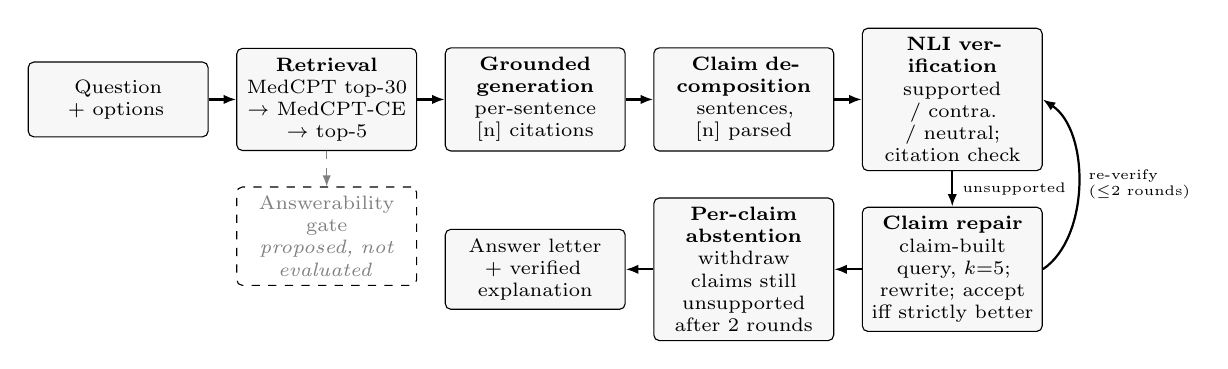
\begin{tikzpicture}[node distance=0.35cm and 0.35cm, every node/.style={font=\scriptsize},
  box/.style={draw, rounded corners=2pt, align=center, minimum height=0.95cm, text width=2.05cm, fill=gray!6},
  gate/.style={draw, dashed, rounded corners=2pt, align=center, minimum height=0.95cm, text width=2.05cm, text=gray},
  arr/.style={-{Latex[length=1.6mm]}, thick}]
\node[box] (q) {Question\\+ options};
\node[box, right=of q] (ret) {\textbf{Retrieval}\\MedCPT top-30 $\to$ MedCPT-CE $\to$ top-5};
\node[gate, below=0.45cm of ret] (g) {Answerability gate\\\emph{proposed, not evaluated}};
\node[box, right=of ret] (gen) {\textbf{Grounded generation}\\per-sentence [n] citations};
\node[box, right=of gen] (dec) {\textbf{Claim decomposition}\\sentences, [n] parsed};
\node[box, right=of dec] (ver) {\textbf{NLI verification}\\supported / contra. / neutral; citation check};
\node[box, below=0.45cm of ver] (rep) {\textbf{Claim repair}\\claim-built query, $k{=}5$; rewrite; accept iff strictly better};
\node[box, left=of rep] (abs) {\textbf{Per-claim abstention}\\withdraw claims still unsupported after 2 rounds};
\node[box, left=of abs] (out) {Answer letter + verified explanation};
\draw[arr] (q) -- (ret); \draw[arr] (ret) -- (gen); \draw[arr] (gen) -- (dec); \draw[arr] (dec) -- (ver);
\draw[arr] (ver) -- node[right, font=\tiny]{unsupported} (rep);
\draw[arr] (rep.east) .. controls +(0.6,0.4) and +(0.6,-0.4) .. node[right, font=\tiny, align=left]{re-verify\\($\le$2 rounds)} (ver.east);
\draw[arr] (rep) -- (abs); \draw[arr] (abs) -- (out);
\draw[dashed, gray, -{Latex[length=1.4mm]}] (ret) -- (g);
\end{tikzpicture}
\caption{Faithful-MedRAG as executed in configuration F. Retrieval feeds five passages to the generator. Each explanation sentence is verified against them. Unsupported sentences are rewritten from evidence retrieved for that sentence, and sentences still unsupported after two rounds are withdrawn individually. The dashed answerability gate is implemented but was not evaluated and is not part of any reported result.}
\label{fig:pipeline}
\end{figure*}

%=====================================================================
\section{Related Work}
%=====================================================================
\subsection{RAG and Medical RAG}
RAG combines a retriever with a generator so that outputs can draw on an external corpus \citep{lewis2020rag}. For biomedicine, MedCPT provides a query/article bi-encoder and a cross-encoder trained on PubMed search logs \citep{jin2023medcpt}. \citet{xiong2024benchmarking} released MIRAGE (7,663 questions from five medical QA datasets) and MedRAG, and reported accuracy for combinations of five corpora, four retrievers, reciprocal rank fusion \citep[RRF;][]{cormack2009rrf} and six LLMs. We reuse MIRAGE, MedCPT and RRF. We add measurements that MIRAGE does not report: claim-level faithfulness and citation correctness.

\subsection{Faithfulness and Attribution Evaluation}
RAGAS scores the faithfulness of RAG outputs without reference answers \citep{es2024ragas}. FActScore decomposes long-form text into atomic facts and checks each against a knowledge source \citep{min2023factscore}. NLI models are a common, inexpensive way to test whether a passage entails a generated statement \citep[e.g.,][]{TODO_true_nli_factuality}, and work on generating text with citations evaluates whether the cited passage supports each statement \citep{TODO_alce_citations}. Our harness uses this NLI-based design at sentence granularity. It reports contradicted and neutral claims separately and scores citation correctness against the \emph{cited} passage rather than against any passage.

\subsection{Corrective and Self-Reflective RAG}
Self-RAG trains a model to emit reflection tokens that critique retrieval need and output support \citep{asai2024selfrag}. CRAG evaluates retrieval quality for a query and triggers corrective actions such as web search \citep{yan2024crag}. Both make decisions for a whole answer or a whole query. Our repair loop acts on the individual claim: it builds the re-retrieval query from the failing sentence, leaves supported sentences untouched, and withdraws only the sentences that cannot be supported.

%=====================================================================
\section{Evaluation Setup}
%=====================================================================
\subsection{Data and Corpus}\label{sec:data}
Table~\ref{tab:resources} lists every resource used. MIRAGE was loaded from its public release and its subset counts match the published counts. % [L01-L06]
Because indexing the 23.9M-snippet MedRAG PubMed corpus exceeded the available disk, we built a documented 43,246-passage corpus. It contains (i) every context section of the 1,000 expert-labelled PubMedQA questions \citep[\texttt{pqa\_labeled};][]{jin2019pubmedqa}, one passage per labelled abstract section, and (ii) a seeded random sample of MedRAG textbook chunks used as in-domain distractors. % [L07-L11]
Passages are de-duplicated on normalised text. This removes 4 of the 3,338 PubMedQA passages and 4 textbook chunks (Table~\ref{tab:resources}). % [L08,L10,L11]

\paragraph{A closed, gold-containing corpus.} The retrieval gold labels are PubMedQA's own context passages, which we deliberately inserted into the corpus. Absolute Recall and MRR therefore describe retrieval from a closed collection in which the relevant passages are known to be present. They are not comparable to open-corpus retrieval. All 500 MIRAGE PubMedQA* questions also have their source abstracts in this corpus, which affects the PubMedQA* cell of Experiment~1 (\S\ref{sec:exp1}). % [L12]

\begin{table}[t]
\centering\small
\setlength{\tabcolsep}{4pt}
\resizebox{\columnwidth}{!}{%
\begin{tabular}{lrl}
\toprule
Resource & Count & Note \\
\midrule
MIRAGE (total) & 7,663 & 5 subsets \\
\quad MedQA-US & 1,273 & \\
\quad MedMCQA & 4,183 & \\
\quad PubMedQA* & 500 & \\
\quad BioASQ-Y/N & 618 & \\
\quad MMLU-Med & 1,089 & \\
\midrule
PubMedQA \texttt{pqa\_labeled} & 1,000 & questions \\
\quad gold passages & 3,338 & 3.34 per question \\
MedRAG textbooks (source) & 125,847 & chunks \\
\quad seeded sample (seed 42) & 40,000 & 39,916 after length filter \\
\midrule
Corpus after de-duplication & 43,246 & \\
\quad from PubMedQA & 3,334 & gold-labelled \\
\quad from textbooks & 39,912 & distractors \\
\bottomrule
\end{tabular}}
\caption{Resources and counts, verified against the data files. Textbook chunks shorter than 50 characters are dropped before de-duplication. PubMedQA* is MIRAGE's question-only version of PubMedQA \citep{xiong2024benchmarking}.} % [L01-L11]
\label{tab:resources}
\end{table}

\subsection{Metrics}\label{sec:metrics}
All definitions follow the implementation (files \texttt{metrics.py} and \texttt{verify.py}).

\paragraph{Retrieval.} For a query with gold passage set $G$ and ranked list $R$,
\begin{equation}
\mathrm{R@}k=\tfrac{|R_{1:k}\cap G|}{|G|},\ \ \mathrm{Hit@}k=\mathbb{1}[R_{1:k}\cap G\neq\emptyset].
\end{equation}
MRR is the reciprocal rank of the first gold passage in the returned list (0 if none is returned). nDCG@$k$ uses binary gains, $\mathrm{DCG@}k=\sum_{i\le k:\,R_i\in G} \log_2^{-1}(i{+}1)$, normalised by the ideal DCG over $\min(|G|,k)$ positions. Retrieval metrics are averaged over queries, with 95\% CIs computed as $1.96\cdot\mathrm{sd}/\sqrt{n}$.

\paragraph{Claim verdicts.} An explanation is split into sentence-level claims $c$. For evidence passages $E=\{e_1,\dots,e_m\}$ the NLI model gives $P_{\text{ent}}(e,c)$ and $P_{\text{con}}(e,c)$, with the passage as premise and the claim as hypothesis. With $\tau_s=\tau_c=0.5$:
\begin{equation}
v(c)=\begin{cases}
\text{sup.} & \text{if } \max_{e}P_{\text{ent}}(e,c)\ge\tau_s,\\
\text{con.} & \text{else if } \max_{e}P_{\text{con}}(e,c)\ge\tau_c,\\
\text{neu.} & \text{otherwise,}
\end{cases}
\end{equation}
with $e$ ranging over $E$ (supported, contradicted, neutral).
\paragraph{Citation correctness.} A claim carrying citation markers $J(c)$ is correctly cited iff
\begin{equation}
\exists j\in J(c):\ P_{\text{ent}}(e_j,c)\ge\tau_s .
\end{equation}
A claim that is entailed by some passage but cites a different one is therefore counted as supported and incorrectly cited. Per answer, \emph{citation precision} is the fraction of cited claims that are correctly cited. The reported value is the mean over answers that contain at least one cited claim.

\paragraph{Faithfulness and hallucination.} Let $S$, $C$, $N$ and $A$ be the numbers of supported, contradicted, neutral and withdrawn (abstained) claims, and let $T=S+C+N+A$ be all claims.
\begin{align}
\mathrm{Faith}_{\text{micro}} &= \textstyle\sum S\,/\,\sum T,\\
\mathrm{Halluc} &= \textstyle\sum (C+N)\,/\,\sum T .
\end{align}
The denominator \emph{includes withdrawn claims}, and the hallucination rate counts only contradicted or neutral claims that \emph{remain in the answer}. $\mathrm{Faith}_{\text{macro}}$ is the mean of the per-answer ratio $S/T$, with a normal-approximation 95\% CI.

\paragraph{Selective metrics.} Coverage is the fraction of questions answered. Selective accuracy is the accuracy over answered questions, and risk is $1-$selective accuracy. A question is unanswered when the grounded generator outputs ``Insufficient evidence'' or when repair withdraws every claim. \emph{Accuracy} (overall) is computed over all questions from the parsed answer letter, including questions whose explanation was withdrawn.

\subsection{Protocol}
All runs use seed 42, greedy decoding (temperature 0) and at most 256 new tokens (Appendix~\ref{app:hyper}). Experiment~1 uses a seeded stratified sample of MIRAGE, with subset shares proportional to subset size. Rounding these shares yields 199 rather than the target 200 questions. % [L13]
The PubMedQA-derived question pool is sorted by question ID. The retrieval bake-off uses all 1,000 questions (\emph{main set}). The reranker diagnostic uses the first 300 (\emph{diagnostic set}). The generation ablation uses the last 200 (\emph{ablation set}), which is disjoint from the diagnostic set but contained in the main set. Each ablation question is posed as a three-option item (A = yes, B = no, C = maybe). % [L14,L15]
Gold labels in the ablation set are 118 yes, 64 no and 18 maybe, so always answering ``yes'' would score 0.590. % [L16]
The recorded run environment is Google Colab with CUDA under Linux (Python 3.13.16, PyTorch 2.14.1, Transformers 5.22.1), and all GPU experiments ran on an NVIDIA T4 GPU provided by Google Colab. The project report states that the MedCPT corpus embedding was computed separately on an Apple M1 (MPS) at 14--17 passages/s, taking about 52 minutes. Timings therefore come from two different environments. % [L17,L18]

%=====================================================================
\section{The Faithful-MedRAG Pipeline}
%=====================================================================
Figure~\ref{fig:pipeline} shows the components that were executed. Table~\ref{tab:components} lists the models.



\begin{table}[t]
\centering\small
\setlength{\tabcolsep}{3pt}
\begin{tabular}{ll}
\toprule
Role & Checkpoint \\
\midrule
Generator & Qwen/Qwen2.5-7B-Instruct \\
Dense retriever & ncbi/MedCPT-Query-Encoder \\
 & ncbi/MedCPT-Article-Encoder \\
Lexical retriever & Okapi BM25 (\texttt{rank\_bm25}) \\
Reranker (proposed) & BAAI/bge-reranker-base \\
Reranker (adopted) & ncbi/MedCPT-Cross-Encoder \\
NLI verifier & MoritzLaurer/DeBERTa-v3- \\
 & \quad base-mnli-fever-anli \\
\bottomrule
\end{tabular}
\caption{Models used \citep{qwen2025qwen25,jin2023medcpt,robertson2009bm25,xiao2023cpack,he2023debertav3,laurer_deberta_nli}. All are public Hugging Face checkpoints. The code requests 4-bit NF4 loading of the generator on CUDA when \texttt{bitsandbytes} is installed.} % [L19]
\label{tab:components}
\end{table}

\subsection{Retrieval}\label{sec:retrieval}
BM25 \citep{robertson2009bm25} indexes lower-cased alphanumeric tokens of ``title. text''. MedCPT \citep{jin2023medcpt} encodes passages as [title, text] pairs with the article encoder and queries with the query encoder (CLS pooling, inner-product scoring). RRF fuses the BM25 and MedCPT lists (30 candidates each) with
\begin{equation}
\mathrm{score}(d)=\sum_{r\in\mathcal{R}}\frac{1}{k+\mathrm{rank}_r(d)},\qquad k=60 .
\end{equation}
In reranked modes, a cross-encoder rescores 30 candidates and returns the top 5 as generation context. The \texttt{medcpt\_ce} mode used from configuration D onward reranks the top 30 \emph{MedCPT} candidates with the MedCPT cross-encoder, without fusion.

\subsection{Grounded Generation}
The vanilla prompt asks for a brief explanation followed by an answer line. The strict-citation prompt adds four rules: (1) every sentence ends with a citation marker [n] naming the supporting document; (2) nothing outside the documents may be stated; (3) the model writes ``Insufficient evidence'' if the documents do not suffice; and (4) each sentence carries one factual claim. The user message asks for 2--4 cited sentences. Full prompts are in Appendix~\ref{app:prompts}. Passages are numbered from 1 and truncated to 900 characters in the prompt.

\subsection{Claim Decomposition and Verification}
The explanation (text before the final ``Answer:'' line) is split into sentences with a regular expression that does not split after common abbreviations (e.g., i.e., vs., Fig.). Citation markers such as [2] or [1, 3] are parsed and removed, and fragments shorter than eight characters are discarded. Each claim is paired with each of the five context passages (truncated to 1,800 characters) and scored by the NLI model. Positions of the entailment and contradiction labels are read from the model's configuration at load time rather than hard-coded. Verdicts and citation correctness follow Eqs.~(2)--(3).

\subsection{Claim-Level Repair and Abstention}\label{sec:repair}
After the first verification, each claim labelled contradicted or neutral is repaired as follows (file \texttt{repair.py}):
\begin{enumerate}
\item \textbf{Targeted query.} Up to 14 distinct content words of the \emph{claim} (stop words removed) are combined with up to six content words of the question, so the query targets the failing proposition.
\item \textbf{Re-retrieval.} Five passages are retrieved with the configuration's retrieval mode. New passages are appended to the existing context and de-duplicated, so citation numbers of already-supported claims stay stable.
\item \textbf{Rewrite.} The generator rewrites only this sentence with the repair prompt (Appendix~\ref{app:prompts}).
\item \textbf{Acceptance.} The rewrite is re-verified against the merged evidence and replaces the original only if it is labelled supported \emph{and} its entailment probability strictly exceeds the original's ($P_{\text{ent}}(c')>P_{\text{ent}}(c)$). A rewrite that says ``Insufficient evidence'' is never accepted.
\end{enumerate}
The loop runs for at most two rounds and stops early once no unsupported claims remain. Every claim still labelled contradicted or neutral afterwards is relabelled \emph{abstained} and dropped from the final answer. If all claims are withdrawn, the explanation is replaced by a fixed insufficient-evidence message and the question counts as unanswered. Supported claims are never rewritten.

%=====================================================================
\section{Results}
%=====================================================================
\paragraph{Verifier sanity probe.} Before running at scale, we checked the verifier on a controlled probe of four claims against two abstracts, as described in the project report (no results file exists for this probe). Two true claims received $P_{\text{ent}}=0.983$ and $0.994$; two fabricated claims received $0.002$ and $0.001$. % [L20]
This shows only that the decision rule behaves sensibly on four hand-made cases. It is not a validation of the verifier, and we draw no accuracy estimate from it.

\subsection{Baseline on a MIRAGE Sample}\label{sec:exp1}
Experiment~1 runs configuration A (MedCPT top-5, vanilla prompt) on 199 MIRAGE questions. Table~\ref{tab:exp1} lists per-subset accuracy beside the published GPT-3.5 MedRAG results. The two rows are \textbf{not comparable}: the setups differ in sample, corpus, generator, retriever and number of retrieved snippets (caption). The macro averages (71.16 vs.\ 71.57) are close by coincidence of two different setups. They do not show that our baseline reproduces or approaches MedRAG. % [L21-L28]
Per-subset samples are small: PubMedQA* has $n=13$ (binomial SD 12.8 points) and BioASQ-Y/N has $n=16$ (SD 9.8). We therefore do not interpret per-subset differences. The PubMedQA* cell is further affected because the source abstracts of these questions are in our corpus (\S\ref{sec:data}). The micro accuracy over all 199 items is 62.31\% (124/199), lower than the macro average because MedMCQA contributes 109 items. For 6 items no answer letter could be parsed, and these count as incorrect. % [L29,L30]

\begin{table}[t]
\centering\small
\setlength{\tabcolsep}{3pt}
\resizebox{\columnwidth}{!}{%
\begin{tabular}{lrrr}
\toprule
Subset & $n$ & Ours (SD) & MedRAG$^\dagger$ \\
\midrule
MMLU-Med & 28 & 82.14 (7.24) & 75.48 \\
MedQA-US & 33 & 72.73 (7.75) & 66.61 \\
MedMCQA & 109 & 50.46 (4.79) & 58.04 \\
PubMedQA* & 13 & 69.23 (12.80) & 67.40 \\
BioASQ-Y/N & 16 & 81.25 (9.76) & 90.29 \\
\midrule
Macro avg. & 199 & 71.16 & 71.57 \\
\bottomrule
\end{tabular}}
\caption{Accuracy (\%) of our configuration-A baseline on a seeded stratified MIRAGE sample. SD is the binomial standard deviation. $^\dagger$GPT-3.5-16k-0613 MedRAG with MedCorp and RRF-4 on all 7,663 questions \citep[Tables 6 and 7]{xiong2024benchmarking}. \textbf{Not directly comparable}: (1) 199 vs.\ 7,663 questions; (2) our 43,246-passage corpus vs.\ MedCorp (30.4M documents / 54.2M snippets; \citealp[Table 3]{xiong2024benchmarking}); (3) Qwen2.5-7B-Instruct vs.\ GPT-3.5; (4) MedCPT alone vs.\ RRF-4. Additionally, we use 5 retrieved passages and a short explanation prompt, whereas MedRAG uses 32 snippets by default with chain-of-thought prompting.} % [L21-L28]
\label{tab:exp1}
\end{table}

\subsection{Retrieval Bake-off}\label{sec:ret}
Table~\ref{tab:ret-main} and Figure~\ref{fig:ret-main} report the four arms originally proposed, on the 1,000-query main set. MedCPT alone has the highest value on every metric (Recall@10 0.782). Fusing it with BM25 lowers Recall@10 to 0.742, and adding the general-domain BGE reranker lowers it further to 0.713. % [L31-L34]
Per-query paired differences confirm both drops. MedCPT$\to$RRF changes Recall@10 by $-0.040$ (bootstrap 95\% CI $[-0.052,-0.028]$; Wilcoxon $p=3.9\times10^{-8}$), and RRF$\to$RRF+BGE by $-0.030$ ($[-0.041,-0.017]$; $p=1.6\times10^{-5}$). BM25 alone reaches Recall@10 0.602, $0.180$ below MedCPT. % [L35-L37]
For the configurations we proposed, these results are negative: neither fusion nor general-domain reranking improved retrieval on this corpus.

\begin{table}[t]
\centering\small
\setlength{\tabcolsep}{2.6pt}
\resizebox{\columnwidth}{!}{%
\begin{tabular}{lcccccc}
\toprule
Mode & R@5 & R@10 & R@20 & MRR & nD@10 & s/q \\
\midrule
BM25 & .552 & .602 & .643 & .888 & .635 & .208 \\
MedCPT & \textbf{.708} & \textbf{.782} & \textbf{.834} & \textbf{.944} & \textbf{.782} & \textbf{.024} \\
RRF & .650 & .742 & .820 & .941 & .743 & .270 \\
RRF+BGE & .635 & .713 & .790 & .921 & .714 & .925 \\
\bottomrule
\end{tabular}}
\caption{Retrieval on the \textbf{main set} ($n=1{,}000$ PubMedQA queries, 43,246-passage closed corpus that contains the gold passages). R@$k$: Recall@$k$; nD@10: nDCG@10; s/q: mean latency in seconds per query. RRF fuses BM25 and MedCPT ($k=60$); BGE is bge-reranker-base over the top-30 fused candidates. 95\% CIs for Recall@10 are $\pm$0.016--0.019 (Appendix~\ref{app:ret}).} % [L31-L34]
\label{tab:ret-main}
\end{table}

\begin{figure*}[t]
\centering
\includegraphics[width=0.9\textwidth]{figures/fig_retrieval_main.pdf}
\caption{Retrieval bake-off on the main set ($n=1{,}000$ queries). Left: Recall@5/10/20; right: MRR and nDCG@10. Error bars are 95\% CIs ($1.96\cdot$sd$/\sqrt{n}$). Data: \texttt{exp3\_retrieval\_bakeoff\_main}.}
\label{fig:ret-main}
\end{figure*}

\subsection{Diagnosing the Regression}\label{sec:diag}
We tested two explanations for the drop on the 300-query diagnostic set (Table~\ref{tab:ret-diag}; Appendix Figure~\ref{fig:ret-diag}).
\textbf{H1, fusion dilution:} RRF weights both lists equally by rank, so a much weaker lexical list can push MedCPT's correct passages down.
\textbf{H2, reranker domain mismatch:} bge-reranker-base is a general-domain cross-encoder, whereas MedCPT's cross-encoder was trained on PubMed search logs \citep{jin2023medcpt}.
To isolate H2, we applied each reranker directly to the MedCPT top-30, without fusion. BGE lowered Recall@10 from 0.762 to 0.693 ($-0.068$, CI $[-0.094,-0.042]$; $p=1.3\times10^{-6}$). The MedCPT cross-encoder raised it to 0.819 ($+0.058$, CI $[0.041,0.075]$; $p=1.3\times10^{-8}$), and MRR from 0.928 to 0.981. Because these runs involve no fusion, the reranker itself explains the BGE loss. % [L38-L43]
For H1, adding RRF in front of the good reranker lowered Recall@10 from 0.819 to 0.804 ($-0.015$). The bootstrap CI $[-0.029,-0.002]$ excludes zero, but the Wilcoxon test does not reach the conventional level ($p=0.076$). We read this as weak evidence that fusion with BM25 still costs a little here. % [L44]
Reranking adds cost: mean latency rises from 0.025\,s to 0.645\,s per query. % [L45]
On the basis of this diagnosis, configurations D--F use MedCPT retrieval with MedCPT cross-encoder reranking, which \emph{replaces} RRF rather than being added to it.
The ablation set itself, retrieved with $k=5$, shows the same ordering of these three modes: Recall@5 is 0.690 for MedCPT (A/B), 0.649 for RRF (C) and 0.792 for MedCPT-CE (D--F) (Table~\ref{tab:ablation-ret}). % [L46]

\begin{table}[t]
\centering\small
\setlength{\tabcolsep}{2.6pt}
\resizebox{\columnwidth}{!}{%
\begin{tabular}{lcccccc}
\toprule
Mode & R@5 & R@10 & R@20 & MRR & nD@10 & s/q \\
\midrule
MedCPT & .682 & .762 & .815 & .928 & .758 & \textbf{.025} \\
MedCPT+BGE & .604 & .693 & .788 & .903 & .686 & .692 \\
MedCPT+CE & \textbf{.765} & \textbf{.819} & \textbf{.836} & \textbf{.981} & \textbf{.831} & .645 \\
RRF+CE & .761 & .804 & .817 & .980 & .822 & .826 \\
\bottomrule
\end{tabular}}
\caption{Reranker diagnosis on the \textbf{diagnostic set} ($n=300$, the first 300 main-set queries; MedCPT values here differ from Table~\ref{tab:ret-main} because the query set differs). CE: MedCPT cross-encoder; BGE: bge-reranker-base; both rerank 30 candidates. Abbreviations as in Table~\ref{tab:ret-main}.} % [L38-L45]
\label{tab:ret-diag}
\end{table}



\subsection{Component Ablation: Accuracy vs.\ Faithfulness}\label{sec:ablation}
Table~\ref{tab:ablation} reports six progressive configurations on the 200-question ablation set. The configurations are not a strict one-component-per-row sequence. A$\to$B is measurement only: the generations are identical (we verified that all 200 answer letters and explanations match), and B adds verification. C switches retrieval to RRF. D \emph{replaces} RRF with MedCPT-CE (\S\ref{sec:diag}). E adds the strict-citation prompt. F adds claim repair and per-claim abstention to E, and leaves E's answer letters and initial explanations unchanged.

\begin{table*}[t]
\centering\small
\setlength{\tabcolsep}{3.4pt}
\resizebox{\textwidth}{!}{%
\begin{tabular}{llcccccccccc}
\toprule
Cfg & Retrieval & Acc. & Cov. & Sel.\,acc. & Faith$_\mu$ & Faith$_M$ ($\pm$CI) & Halluc. & Cit.\,prec. & Claims & Rep./Withdr. & s/q \\
\midrule
A vanilla & MedCPT & .595 & 1.000 & .595 & -- & -- & -- & -- & -- & 0 / 0 & 6.01 \\
B +verification & MedCPT & .595 & 1.000 & .595 & .593 & .589 $\pm$.041 & .407 & .742$^{a}$ & 578 & 0 / 0 & 5.82 \\
C +RRF & RRF & .610 & 1.000 & .610 & .625 & .619 $\pm$.041 & .375 & .744$^{a}$ & 582 & 0 / 0 & 6.09 \\
D MedCPT-CE (repl.\ RRF) & MedCPT-CE & .645 & 1.000 & .645 & .622 & .613 $\pm$.041 & .378 & .703$^{a}$ & 588 & 0 / 0 & 6.35 \\
E +strict citation & MedCPT-CE & .645 & .975 & .656 & .518 & .520 $\pm$.046 & .482 & .491 & 558 & 0 / 0 & 7.04 \\
F +claim repair & MedCPT-CE & .645 & .895 & .654 & .651 & .652 $\pm$.044 & .000$^{b}$ & .586 & 558 & 74 / 195 & 16.81 \\
\bottomrule
\end{tabular}}
\caption{Progressive configurations on the \textbf{ablation set} ($n=200$ PubMedQA-derived three-option questions; majority-class accuracy 0.590). Acc.: accuracy over all 200 questions, including those whose explanation was withdrawn (95\% CI $\pm$.066--.068). Cov.: coverage. Sel.\,acc.: accuracy on answered questions. Faith$_\mu$/Faith$_M$: micro/macro claim faithfulness (Eq.~4; withdrawn claims stay in the denominator). Halluc.: contradicted + neutral claims remaining in the answer / all claims. Cit.\,prec.: mean per-answer citation precision. Rep./Withdr.: claims repaired / withdrawn. s/q: mean end-to-end seconds per question. $^{a}$Computed only over the 44 (B), 52 (C) and 30 (D) answers in which the vanilla prompt produced any citation; E and F are computed over 169 answers. $^{b}$Zero because all 195 claims (34.9\%) still unsupported after two repair rounds were withdrawn, not because they were corrected; coverage falls to 0.895 as a result.} % [L47-L66]
\label{tab:ablation}
\end{table*}

\paragraph{Accuracy.} Accuracy ranges from 0.595 (A, B) to 0.645 (D--F). The A$\to$D difference lies within the 95\% CI. An exact McNemar test on the paired answers finds no significant difference (23 questions correct only under D vs.\ 13 only under A; $p=0.13$). Neither does C vs.\ D ($p=0.21$). All configurations are close to the 0.590 majority-class rate. % [L47,L67-L69]
\paragraph{Faithfulness.} Under the vanilla prompt, faithfulness changes little across retrieval modes. Paired bootstrap 95\% CIs (10,000 resamples of questions) for the micro difference include zero for B$\to$C ($+3.2$ points, CI $[-1.6,8.1]$) and B$\to$D ($+2.9$, $[-1.8,7.6]$). % [L70,L71]
The strict-citation prompt \emph{lowers} faithfulness from 0.622 (D) to 0.518 (E), a change of $-10.5$ points (CI $[-15.5,-5.5]$). Its neutral rate rises from 0.338 to 0.428 (Figure~\ref{fig:breakdown}). % [L72,L73]
Repair raises faithfulness from 0.518 (E) to 0.651 (F), $+13.3$ points (CI $[10.2,16.7]$). Relative to the vanilla-prompt baseline B, F is $+5.7$ points (CI $[0.1,11.3]$). Relative to D, the best configuration without repair and with the same retriever, F is $+2.8$ points (CI $[-2.2,7.9]$), which is not significant. % [L74-L76]
Most of the E$\to$F gain therefore recovers the loss that the strict-citation prompt introduced.

\begin{figure}[t]
\centering
\includegraphics[width=\columnwidth]{figures/fig_claim_breakdown.pdf}
\caption{Claim verdicts by configuration on the ablation set ($n=200$ questions; total claims above each bar). In F, ``withdrawn'' claims are those still unsupported after two repair rounds. They are why F's hallucination rate is 0 (195 of 558 claims withdrawn). Data: \texttt{ablation\_configurations}.}
\label{fig:breakdown}
\end{figure}

\subsection{What Accuracy Cannot See}\label{sec:cannotsee}
D, E and F have the same accuracy, 0.645. E and F also have identical answer letters, because F changes only the explanation. Their claim-level profiles differ markedly (Figure~\ref{fig:scatter}). Micro faithfulness is 0.622, 0.518 and 0.651, and citation precision is 0.703, 0.491 and 0.586. An accuracy-only evaluation would rate D, E and F as equivalent. A claim-level evaluation shows that E's explanations contain the most unsupported content and that F's contain the least that remains asserted. % [L77]

\begin{figure}[t]
\centering
\includegraphics[width=\columnwidth]{figures/fig_acc_vs_faith.pdf}
\caption{Accuracy vs.\ micro claim faithfulness for configurations B--F on the ablation set ($n=200$). Horizontal bars are 95\% CIs for accuracy. A is omitted because it is not verified. D, E and F share accuracy 0.645 but span 0.518--0.651 in faithfulness. Data: \texttt{ablation\_configurations}.}
\label{fig:scatter}
\end{figure}

%=====================================================================
\section{Discussions}
%=====================================================================
\subsection{Accuracy Is Not Faithfulness}
On this evaluation, the answer letter and the explanation behave as largely separate outputs. Changing the prompt moved faithfulness by 10.5 points without changing accuracy (D$\to$E: 13 questions gained and 13 lost, McNemar $p=1.0$), and repair moved it by 13.3 points with no change to any answer letter. % [L72,L74,L78]
Reporting only accuracy, as MIRAGE-style evaluations do, cannot detect either effect. We consider claim-level measurement a necessary complement to accuracy. Its validity, however, depends on a verifier that we have not yet validated against human judgments (Limitations).

\subsection{Why Fusion Failed Here}
\citet[Table 7]{xiong2024benchmarking} report that, with GPT-3.5 on the PubMed corpus, BM25 and MedCPT yield near-equal average MIRAGE accuracy (69.23 vs.\ 69.38). In their setting, RRF-2 (BM25 + MedCPT) exceeded both of its component retrievers on all five corpora. % [L79,L80]
On our corpus the two retrievers are far from equal: Recall@10 is 0.602 for BM25 and 0.782 for MedCPT on the main set. Uniform rank fusion lowered recall. We hypothesise that RRF helps when its inputs are comparably strong and hurts when one input is much weaker. This difference in relative strength may in turn reflect our small, textbook-dominated closed corpus. We did not test this hypothesis. Note also that the published parity concerns end-task accuracy, whereas our comparison concerns retrieval recall. Testing it would require the full PubMed corpus, or weighted or learned fusion.

\subsection{The Cost of Faithfulness}\label{sec:cost}
The repair loop's gains have four costs that a reader of Table~\ref{tab:ablation} should weigh.
(i) \textbf{Withdrawal, not correction.} Of the 558 claims in F, 74 were repaired and 195 (34.9\%) were withdrawn. F's hallucination rate of 0 holds by construction: unsupported claims are removed, not fixed. % [L59-L61]
(ii) \textbf{Coverage.} 21 of 200 answers (coverage 0.895) are unanswered. In 17 of them repair withdrew every claim, and in 4 the generator itself declared insufficient evidence. Under our accuracy definition, 12 of these 21 still carry a correct answer letter. % [L62,L63]
(iii) \textbf{Citation precision.} Strict citation lowered citation precision from 0.703 (D) to 0.491 (E). Repair recovered it only to 0.586 (F), which remains below B--D. The B--D values are, however, computed over the 30--52 answers in which the vanilla prompt chose to cite, whereas E/F are computed over 169 answers, so the populations differ. % [L64]
(iv) \textbf{Latency.} Mean time per question rises from 7.04\,s (E) to 16.81\,s (F). Repair alone takes 9.68\,s per question on average and makes 468 targeted re-retrievals (Appendix Figure~\ref{fig:latency}). % [L65,L66]

Inspecting F's outputs reveals further failure modes. In 24 of 200 final explanations, the literal placeholder ``[n]'' from the prompt appears instead of a passage number. Accepted rewrites sometimes restate a passage rather than the inference the original sentence made. In Appendix~\ref{app:example}, the withdrawn claim is the one that carried the answer to the question. % [L81]
Repair thus favours statements that the evidence supports over statements that answer the question.

\subsection{Practical Recommendations}
The following are supported by our results, within this setting (a 43k closed corpus, a 7B generator, and $n\le1{,}000$ queries):
\begin{itemize}
\item \textbf{Report claim-level faithfulness next to accuracy.} Configurations with equal accuracy differed by up to 13.3 faithfulness points.
\item \textbf{Validate a reranker in-domain before adopting it.} The general-domain BGE reranker lowered recall here; the biomedical MedCPT cross-encoder raised it.
\item \textbf{Measure component retrievers before fusing them.} Uniform RRF with a much weaker lexical retriever lowered recall on this corpus.
\item \textbf{Never report a post-abstention hallucination rate alone.} Report it together with the withdrawal rate and coverage.
\item \textbf{Verify, rather than assume, the effect of citation prompts.} With a 7B generator, the strict-citation prompt lowered both faithfulness and citation precision.
\end{itemize}

%=====================================================================
\section{Conclusion}
%=====================================================================
We built and evaluated a claim-level verification and repair pipeline for biomedical RAG. On a closed 43k-passage corpus, MedCPT outperformed BM25 and RRF fusion, and a domain-matched cross-encoder improved on MedCPT where a general-domain reranker did not. On 200 PubMedQA-derived questions, accuracy did not distinguish configurations whose claim faithfulness differed by up to 13.3 points. Claim-level repair raised faithfulness over the strict-citation configuration, mainly by withdrawing unsupported claims and at a clear cost in coverage and latency. Future work will evaluate the learned answerability gate (a pre-generation classifier over 13 retrieval-score and query--evidence NLI features), run the full 7,663-question MIRAGE benchmark, test out-of-distribution generalisation on MedQA/USMLE, and validate the NLI verifier against human judgments.

\section*{Limitations}
\textbf{Sample sizes.} The ablation uses 200 questions and the diagnostic retrieval study 300. Per-subset MIRAGE cells have as few as 13 items. Accuracy CIs ($\pm$0.066--0.068) are wide relative to the differences we observe, and only the E$\to$F, D$\to$E and B$\to$F faithfulness differences have bootstrap CIs that exclude zero (B$\to$F only narrowly).
\textbf{Closed, gold-containing corpus.} Gold passages were inserted into the corpus, so retrieval and grounding are easier than in open-corpus retrieval over PubMed. The configuration choice for D--F was made on the diagnostic set, which is disjoint from the ablation set; the main retrieval set, however, overlaps the ablation set.
\textbf{Single generator.} All generation used Qwen2.5-7B-Instruct with greedy decoding; results may not transfer to other or larger models.
\textbf{Verifier not validated.} The NLI verifier (DeBERTa-v3-base-mnli-fever-anli, max-over-passages entailment) has not been validated against human judgments in this work. The four-claim probe is only a sanity check. All faithfulness, hallucination and citation numbers inherit the verifier's unknown error rate.
\textbf{Claim granularity.} A sentence is not an atomic claim. A sentence with one supported and one unsupported proposition receives a single verdict.
\textbf{Multi-passage synthesis.} Max-over-passages entailment cannot credit a claim whose support is spread across several passages, so such claims are labelled neutral and may be withdrawn.
\textbf{Metric conventions.} Overall accuracy still credits the answer letter of withdrawn answers. Citation precision for the vanilla prompt rests on few answers.
\textbf{Latency.} Mean latencies include the first, warm-up item of each run and were measured on a single Colab T4 GPU.
\textbf{Not yet executed.} The learned answerability gate, out-of-distribution evaluation, human evaluation, the faithfulness--helpfulness trade-off study, ablation configurations G/H and the full MIRAGE run were not executed. No claim in this paper depends on them.
\textbf{Repair trade-offs.} Repair can trade citation precision and informativeness for entailment, and it occasionally emits malformed citations.

\section*{Ethics Statement}
This system is a research prototype and has not been evaluated for clinical use. It must not be used to inform patient care. All datasets and models are publicly released, and our code, results and analysis scripts are available at \url{https://github.com/Veeralpatidar/Faithful-MedRAG}. No human subjects or private data were involved.

\IfFileExists{acl_natbib.bst}{\bibliographystyle{acl_natbib}}{\bibliographystyle{plainnat}}
\bibliography{references}

\appendix
\onecolumn
\section{Prompt Templates}\label{app:prompts}
Figures~\ref{fig:prompt-vanilla}--\ref{fig:prompt-repair} reproduce the three prompt pairs. Context passages are formatted as \texttt{[i] (title) text}, with text truncated to 900 characters and passages separated by blank lines.
\input{prompts_appendix.tex}
\clearpage

\section{Hyperparameters and Provenance}\label{app:hyper}
\begin{table}[h]
\centering\small
\begin{tabular}{ll@{\qquad}ll}
\toprule
Parameter & Value & Parameter & Value \\
\midrule
\texttt{k\_dense} & 30 & \texttt{max\_repair\_rounds} & 2 \\
\texttt{k\_lexical} & 30 & \texttt{k\_repair\_retrieve} & 5 \\
\texttt{rrf\_k} & 60 & \texttt{max\_new\_tokens} & 256 (repair: 96) \\
\texttt{k\_rerank\_in} & 30 & \texttt{temperature} & 0.0 (greedy) \\
\texttt{k\_context} & 5 & seed & 42 \\
NLI support threshold $\tau_s$ & 0.5 & \texttt{embed\_batch\_size} & 256 \\
NLI contradict threshold $\tau_c$ & 0.5 & \texttt{rerank\_batch\_size} & 64 \\
\texttt{gate\_threshold} (unused) & 0.5 & \texttt{nli\_batch\_size} & 64 \\
\midrule
corpus profile & \texttt{subset\_textbooks} & generator profile & \texttt{proposal\_7b} \\
environment & Colab, CUDA (NVIDIA T4) & platform & Linux-6.6.159+-x86\_64 \\
Python & 3.13.16 & PyTorch & 2.14.1+cu130 \\
Transformers & 5.22.1 & scikit-learn / NumPy / pandas & 1.6.1 / 2.4.6 / 2.2.3 \\
\bottomrule
\end{tabular}
\caption{Values from the \texttt{provenance} sheet of the results workbook. The repair-call token limit (96) and the 900/1,800-character passage truncation for generation/NLI are taken from the code.} % [L82]
\end{table}

\section{Experiment 1 Details}\label{app:exp1}
The stratified sample takes $\mathrm{round}(200\cdot|s|/7{,}663)$ questions from each subset $s$ (MMLU-Med 28, MedQA-US 33, MedMCQA 109, PubMedQA* 13, BioASQ-Y/N 16; 199 in total) with seed 42. Binomial SDs are $\sqrt{a(1-a)/n}$. Mean end-to-end latency is 7.37\,s per question, including a 207\,s first item. For reference, \citet[Table 7]{xiong2024benchmarking} report 60.69 average accuracy for GPT-3.5 without retrieval (chain-of-thought). We did not run a no-retrieval baseline. % [L83,L84]

\section{Extended Retrieval Metrics}\label{app:ret}
\begin{table}[h]
\centering\small
\begin{tabular}{llcccccccc}
\toprule
Set & Mode & Hit@5 & Hit@10 & Hit@20 & nDCG@5 & nDCG@20 & R@10 CI & dense s & rerank s \\
\midrule
Main & BM25 & .933 & .948 & .963 & .616 & .650 & $\pm$.019 & -- & -- \\
Main & MedCPT & .979 & .988 & .994 & .752 & .802 & $\pm$.016 & .024 & -- \\
Main & RRF & .974 & .987 & .993 & .706 & .772 & $\pm$.017 & .022 & -- \\
Main & RRF+BGE & .969 & .986 & .992 & .683 & .742 & $\pm$.017 & .023 & .654 \\
\midrule
Diag & MedCPT & .980 & .987 & .993 & .727 & .778 & $\pm$.029 & .025 & -- \\
Diag & MedCPT+BGE & .977 & .987 & .993 & .651 & .720 & $\pm$.030 & .023 & .658 \\
Diag & MedCPT+CE & .990 & .993 & .993 & .813 & .838 & $\pm$.026 & .023 & .584 \\
Diag & RRF+CE & .987 & .990 & .990 & .810 & .827 & $\pm$.027 & .023 & .574 \\
\bottomrule
\end{tabular}
\caption{Hit@$k$, nDCG@5/20, Recall@10 95\% CI half-width and per-stage mean latency (s/query). BM25 lexical time is 0.208 (main, BM25), 0.248 (RRF), 0.234 (RRF+BGE) and 0.228\,s (diag, RRF+CE). Main $n=1{,}000$, diag $n=300$.} % [L85]
\label{tab:ret-ext}
\end{table}

\begin{table}[h]
\centering\small
\begin{tabular}{lcccc}
\toprule
Retrieval mode (configs) & Recall@5 & Hit@5 & nDCG@5 & MRR \\
\midrule
MedCPT (A, B) & .690 & .975 & .732 & .925 \\
RRF (C) & .649 & .990 & .710 & .965 \\
MedCPT-CE (D--F) & .792 & 1.000 & .835 & .990 \\
\bottomrule
\end{tabular}
\caption{Retrieval quality of the five context passages actually given to the generator, on the \textbf{ablation set} ($n=200$). Only five passages are retrieved, so Recall@10/20 equal Recall@5.} % [L46]
\label{tab:ablation-ret}
\end{table}

\begin{figure}[h]
\centering
\includegraphics[width=0.45\textwidth]{figures/fig_latency.pdf}
\caption{Mean end-to-end latency per question by stage on the ablation set ($n=200$); totals above bars. Verification and retrieval times are small (0.10--0.13\,s and 0.02--0.62\,s). Data: \texttt{ablation\_configurations}.}
\label{fig:latency}
\end{figure}

\begin{figure*}[h]
\centering
\includegraphics[width=0.9\textwidth]{figures/fig_retrieval_diag.pdf}
\caption{Reranker diagnosis on the diagnostic set ($n=300$ queries). CE: MedCPT cross-encoder. Error bars are 95\% CIs. Data: \texttt{exp3\_retrieval\_bakeoff\_rerank\_diag}.}
\label{fig:ret-diag}
\end{figure*}

\section{Worked Example of Claim Repair}\label{app:example}
The following is taken verbatim from \texttt{ablation\_per\_item}, question \texttt{pubmedqa\_src:25604390} (gold answer ``yes''; predicted A = yes). In configuration F it has 2 claims: 1 repaired, 1 withdrawn, 2 repair rounds, faithfulness 0.5. % [L86]

\noindent\textbf{Initial explanation (configuration E/F, before repair):}
\begin{quote}\small
Loss of DKK3 expression was found in 40.5\% of the samples and was associated with lymph node metastasis [1]. This indicates that DKK3 loss can predict lymph node metastasis preoperatively [1].
\end{quote}
\textbf{Final explanation after repair (configuration F):}
\begin{quote}\small
Loss of DKK3 expression was found in 64 of 158 (40.5\%) samples and was associated with lymph node metastasis (p<0.001) . [1]
\end{quote}
The first claim was rewritten into a more specific sentence that the verifier accepts. The second claim, an inference that directly answers the question, could not be supported after two rounds and was withdrawn. The answer letter (``yes'') is unchanged. The example shows the mechanism working as designed, and also how repair can remove the sentence that connects the evidence to the answer.

\end{document}
